% $Header: /home/vedranm/bitbucket/beamer/solutions/generic-talks/generic-ornate-15min-45min.en.tex,v 90e850259b8b 2007/01/28 20:48:30 tantau $
\documentclass{beamer}
%\documentclass[handout]{beamer}
\usefonttheme[onlymath]{serif}
% This file is a solution template for:
\usepackage{algcompatible}
\usepackage{algpseudocode}
\usepackage{multicol}
% - Giving a talk on some subject.
% - The talk is between 15min and 45min long.
% - Style is ornate.



% Copyright 2004 by Till Tantau <tantau@users.sourceforge.net>.
%
% In principle, this file can be redistributed and/or modified under
% the terms of the GNU Public License, version 2.
%
% However, this file is supposed to be a template to be modified
% for your own needs. For this reason, if you use this file as a
% template and not specifically distribute it as part of a another
% package/program, I grant the extra permission to freely copy and
% modify this file as you see fit and even to delete this copyright
% notice. 

\mode<presentation>
{
  \usetheme{Warsaw}
  % or ...

  \setbeamercovered{transparent}
  % or whatever (possibly just delete it)
}
\setbeamertemplate{navigation symbols}{} 

\usepackage[english]{babel}
% or whatever

\usepackage[latin1]{inputenc}
% or whatever
\useoutertheme{default}

\usepackage{times}
\usepackage[T1]{fontenc}
% Or whatever. Note that the encoding and the font should match. If T1
% does not look nice, try deleting the line with the fontenc.
\newcommand{\beforeverb}{\scriptsize}
\newcommand{\afterverb}{\normalsize}

\title[Ordinary Differential Equations] % (optional, use only with long paper titles)
{Lecture 11}

\subtitle
{Ordinary Differential Equations} % (optional)

\author[Ying-Jer Kao] % (optional, use only with lots of authors)
{Ying-Jer Kao}
% - Use the \inst{?} command only if the authors have different
%   affiliation.

\institute[National Taiwan University] % (optional, but mostly needed)
{
  Department of Physics\\
 National Taiwan University
  }
% - Use the \inst command only if there are several affiliations.
% - Keep it simple, no one is interested in your street address.

\date[Numerical Analysis and Programming] % (optional)
{\today}

\subject{Talks}
% This is only inserted into the PDF information catalog. Can be left
% out. 



% If you have a file called "university-logo-filename.xxx", where xxx
% is a graphic format that can be processed by latex or pdflatex,
% resp., then you can add a logo as follows:

% \pgfdeclareimage[height=0.5cm]{university-logo}{university-logo-filename}
% \logo{\pgfuseimage{university-logo}}



% Delete this, if you do not want the table of contents to pop up at
% the beginning of each subsection:
%\AtBeginSubsection[]
%{
%  \begin{frame}<beamer>{Outline}
%    \tableofcontents[currentsection,currentsubsection]
%  \end{frame}
%}


% If you wish to uncover everything in a step-wise fashion, uncomment
% the following command: 

%\beamerdefaultoverlayspecification{<+->}


\begin{document}

\begin{frame}
  \titlepage
\end{frame}

\begin{frame}{Outline}
  \tableofcontents
  % You might wish to add the option [pausesections]
\end{frame}


% Since this a solution template for a generic talk, very little can
% be said about how it should be structured. However, the talk length
% of between 15min and 45min and the theme suggest that you stick to
% the following rules:  

% - Exactly two or three sections (other than the summary).
% - At *most* three subsections per section.
% - Talk about 30s to 2min per frame. So there should be between about
%   15 and 30 frames, all told.
\section[Introduction]{Introduction}
\begin{frame}{Introduction}
\begin{itemize}
\item An \alert{ordinary differential equation} (ODE) is an equation that involves one or more derivatives of an unknown function. 
\item A \alert{solution} of a differential equation is a specific function that satisfies the equation.
\begin{align*}
x'-x&=e^t &x(t)&=te^t + c e^t\\
x''+9x&=e^t&x(t)&=c_1\sin3t+c_2 \cos 3t\\
x'+\frac{1}{2x}&=0 &x(t)&=\sqrt{c-t}
\end{align*}
\item The constants $c, c_1, c_2$ are determined by the \alert{initial conditions}. 
 \end{itemize}
\end{frame}

\begin{frame}{Initial-Value Problem}
\begin{itemize}
\item We focus on the initial-value problem for a \alert{first-order} ODE, 
%\beforeverb
\[
x'=f(x(t),t); \quad x(a)=s
\]
%\[
%\left\{
%\begin{split}
%\frac{dx}{dt}&=f(x,t)\\ 
%x(a) &= s
%\end{split}\right.
%\]
\afterverb 
\item A numerical solution of a differential equation is usually obtained in the form of a \alert{table}; the functional form of the solution remains unknown.
\item Solving ordinary differential equations numerically requires a \alert{large number of steps} with \alert{small step size}, so a significant amount of \alert{roundoff error can accumulate}. 
\end{itemize}
\end{frame}

\begin{frame}{Vector Fields}
\begin{itemize}
\item Consider a generic first-order differential equation,
\beforeverb
%\[
%\frac{dx}{dt}=f(x,t);\quad x(a)=s
%\]
\[
\left\{
\begin{split}
\frac{dx}{dt}&=f(x,t)\\ 
x(a) &= s
\end{split}\right.
\]
\afterverb
\item To get some intuition, we first visualize the \alert{vector field} of the equation.
\item In the $tx$-plane, at every point $f(x, t)$ is defined, we plot a line segment having the slope $x'=f(x,t)$. 
\item We hope to understand how the \alert{ solution function $x(t)$} evolves through these line segments  while keeping its slope  to the slope of the line segment drawn at that point.
\end{itemize}
\end{frame}


\begin{frame}{Vector Fields}
\centerline{\includegraphics[width=0.8\textwidth]{Lec13_fig1}}
\begin{center}
$x'=\sin(x+t^2)$
\end{center}
\end{frame}
\begin{frame}{Vector Fields}
\centerline{\includegraphics[width=0.8\textwidth]{Lec13_fig2}}
\begin{center}
$x'=x^2-t$, very sensitive to the initial condition!!
\end{center}
\end{frame}

\begin{frame}{Solving Differential Equations and Integration}
\begin{itemize}
\item Consider a generic first-order ODE:
$\frac{dx}{dr}=f(x(r),r)$. 
\item Integrating from $t$ to $t+h$, 
\beforeverb
\begin{align*}
\int_t^{t+h} dx&=\int_t^{t+h} f(x(r),r) dr\\
x(t+h)&=x(t)+\int_t^{t+h} f(x(r),r) dr
\end{align*}
\afterverb

\item Replacing the integral with one of the numerical integration rules, we obtain a formula for solving the differential equation.
\item For example, using the trapezoidal rule, we obtain the \alert{implicit formula},
\beforeverb
\[
x(t+h)=x(t)+\frac{h}{2}\left[f(x(t),t)+f(x(t+h), t+h)\right]
\]
\afterverb
\end{itemize}
\end{frame}


\section[Taylor Series Methods]{Taylor Series Methods }
\begin{frame}{Taylor Series Methods}

\begin{itemize}
\item Assume the solution function $x(t)$ can be represented by a Taylor series
\beforeverb
\[
x(t+h)=x(t)+h x'(t)+\frac{h^2}{2!}x''(t)+\frac{h^3}{3!}x'''(t)+\frac{h^4}{4!}x^{(4)}(t) +\cdots+\frac{h^m}{m!}x^{(m)}(t)+\cdots
\]
\afterverb
\item The Taylor series truncated after $m+1$ terms enables us to compute $x(t+h)$ rather accurately if $h$ is small and if $x(t),x'(t),x''(t),...,x^{(m)}(t)$ are known. This is called the \alert{Taylor series method of order $m$}.
\item The methods based on Taylor series are the most \alert{general}, and it is capable of \alert{high precision}. 	
\end{itemize}
\end{frame}


\subsection[Euler's Method]{Euler's Method}
\begin{frame}{Euler's Method}

\begin{itemize}
\item The Taylor series method of order one ($m=1$) is called the \alert{Euler's method}.
\item To find the solution of the initial-value problem over the interval $[a,b]$,
\beforeverb
\[
\frac{dx}{dt}=f(x,t);\quad x(a)=x_a
\]
\afterverb
\item Using $x(t+h)\approx x(t)+hx'(t)$, we obtain 
\[
x(t+h)=x(t)+hf(x(t),t)
\]
which can be used to step from $t=a$ to $t=b$ with $n$ steps of size $h=(b-a)/n$.
\item Truncation error: $O(h^2)$.
\end{itemize}
\end{frame}

\begin{frame}{Euler's Method: Pseudo Code}
%\beforeverb
\begin{block}{Euler's Method}
\begin{algorithmic}[1]
\State \textbf{integer}: $k$, \textbf{real}:$h, t$
\State $n\gets 100$
\State \textbf{external function} $f$
\State $a\gets 1, b  \gets 2, x\gets -4$
\State $h\gets  (b-a)/n$
\State $t\gets a $
\State \textbf{output} $0,t,x$
\For {$k \gets 1, n$} 
\State $x \gets x+hf(x,t)$
\State $t\gets t+h$
\State \textbf{output} $k,t,x$
\EndFor
\end{algorithmic}
\end{block}
%\afterverb

\end{frame}

\subsection[Taylor Series Method of Order 4]{Taylor Series Method of Order 4}
\begin{frame}{Taylor Series Method of Order 4}
\begin{itemize}
\item Consider the initial value problem,
\[
\left\{
\begin{split}
x'&=1+x^2 +t^3\\ 
x(1) &= -4
\end{split}\right.
\]
\item Differentiation of the equation several times, we obtain
\begin{align*}
x'&=1+x^2+t^3\\
x''&=2xx'+3t^2\\
x'''&=2xx''+2(x')^2+6t\\
x^{(4)}&= 2xx'''+6x'x''+6
\end{align*}
\end{itemize}

\end{frame}

\begin{frame}{Taylor Series Method of Order 4}
\begin{itemize}
\item If numerical values of $t$ and $x(t)$ are known, these four formulas, applied in order, yield $x'(t), x''(t), x'''(t)$, and $x^{(4)}(t)$.
\item We can use the first \alert{five} terms in the Taylor series
\[
x(t+h)= x(t)+h\left[x'(t)+\frac{1}{2}h\left[x''(t)+\frac{1}{3}h\left[x'''(t)+\frac{1}{4}hx^{(4)}(t)\right]\right]\right]
\]
\end{itemize}

\end{frame}

\begin{frame}{Taylor Series Method of Order 4: Pseudo Code}
\beforeverb
\begin{block}{Taylor Series Method of Order 4}
\begin{algorithmic}
\State \textbf{integer}: $k$, \textbf{real}:$h, t, x, x', x'', x''', x^{(4)}$
\State $n\gets 100$
\State \textbf{external function} $f$
\State $a\gets 1, b  \gets 2, x\gets -4$
\State $h\gets  (b-a)/n$
\State $t\gets a $
\State \textbf{output} $0,t,x$
\For {$k \gets 1, n$} 
\State $x' \gets 1+x^2+t^3$
\State $x'' \gets 2xx'+3t^2$
\State $x'''=2xx''+2(x')^2+6t$
\State $x^{(4)}= 2xx'''+6x'x''+6$
\State $x\gets x+h\left[x'+\frac{1}{2}h\left[x''+\frac{1}{3}h\left[x'''+\frac{1}{4}hx^{(4)}\right]\right]\right]$
\State $t\gets t+h$
\State \textbf{output} $k,t,x$
\EndFor
\end{algorithmic}
\end{block}
\afterverb

\end{frame}
\begin{frame}{Error Estimate}
\begin{itemize}

\item At each step, if $x(t)$ is known and $x(t +h)$ is computed from the first few terms of the Taylor series, an error occurs due to truncation. This is the \alert{local truncation error}.
 \item Euler method has truncation error of $O(h^2)$. Taylor series method of order 4 has  the truncation error of $O(h^5)$.
\item Another type of error is due to the \alert{accumulated effects} of all local truncation errors. 
\item The calculated value of $x(t + h)$ is in error because 
\begin{itemize} 
\item $x(t)$ is in error due to \alert{previous truncation errors},
\item \alert{local truncation error} occurs in the computation of $x(t + h)$.
\end{itemize} 

\item Roundoff error may not be serious in \alert{a single step} of the solution process. After hundreds or thousands of steps, though, it may accumulate and seriously contaminate the calculated solution.
 
\end{itemize}
\end{frame}
\section[Runge-Kutta Methods]{Runge-Kutta Methods}
\begin{frame}{Runge-Kutta Methods}
\begin{itemize}
\item In Taylor series methods, we need to compute $x'',x''',\ldots$ by differentiating the function $f$.
\item This requires \alert{pre-computation} of these derivatives analytically before coding.
\item Ideally, a method should involve only the evaluation of $f$. 
\item The  Runge-Kutta methods are designed to imitate the Taylor series method \alert{without} requiring analytic differentiation of the original differential equation.
\end{itemize}
\end{frame}
\subsection[Runge-Kutta Method of Order 2]{Runge-Kutta Method of Order 2}
\begin{frame}{Runge-Kutta Method of Order 2}
\begin{itemize}
\item Consider the functions $K_1, K_2$, 
\[
K_1 = h f(t,x),\quad K_2 =h f(t+\alpha h, x+\beta K_1),
\]
and the value of $x$ at $t+h$ 
\begin{align*}
x(t+h)&=x(t)+w_1K_1+w_2 K_2\\
&=x(t)+w_1hf(t,x)+w_2h f(t+\alpha h, x+\beta h f(t,x))
\end{align*}
\item We want to determine $w_1, w_2, \alpha,\beta$ so the solution is \alert{accurate}, i.e., reproducing as many terms as possible in Taylor series,
\[
x(t+h)=x(t)+h x'(t)+\frac{h^2}{2!}x''(t)+\frac{h^3}{3!}x'''(t) +\cdot
\]
\item By the choice of $w_1=1$ and $w_2=0$ reproduces Euler's method, which agrees to the order $h$.
\end{itemize}
\end{frame}
\begin{frame}{Runge-Kutta Method of Order 2}
\begin{itemize}
\item Expand $f(t+\alpha h, x+\beta h f)$ near $(t,x)$
\[
f(t+\alpha h, x +\beta h f) = f+\alpha h f_t +\beta h f f_x + \frac{1}{2}\left(\alpha h \frac{\partial }{\partial t} +\beta h f \frac{\partial }{\partial x} \right) ^2 f(\bar{t},\bar{x})
\]
\item The solution $x(t+h)$ is 
\[
x(t+h)=x(t)+(w_1+w_2) hf +\alpha w_2 h^2 f_t + \beta w_2 h^2 f f_x +O(h^3)
\]
\item Taylor series up to $h^2$ order, rewrite $x''=f_t+f_x f$ using $x'=f$, 
\[
x(t+h)=x +h f +\frac{1}{2}h^2 f_t +\frac{1}{2} h^2 f f_x +O(h^3)
\]
\item The equations for $w_1, w_2, \alpha, \beta$ are
\[
w_1+w_2=1, \quad \alpha w_2 = \frac{1}{2},  \quad \beta w_2 =\frac{1}{2}. 
\]
\end{itemize}
\end{frame}

\begin{frame}{Runge-Kutta Method of Order 2}
\begin{itemize}
\item A solution (\alert{Heun's method}) is 
\beforeverb
\[
\alpha=1\quad \beta=1 \quad w_1=w_2=\frac{1}{2}
\]
\afterverb
and we obtain \alert{second-order Runge-Kutta method},
\[
x(t+h)=x(t)+\frac{h}{2}f(t,x)+\frac{h}{2}f(t+h,x+hf(t,x))
\]
The solution  is computed with \alert{two evaluations} of $f(t,x)$.
\item Other solutions are possible. For arbitrary $\alpha$, 
\beforeverb
\[
\beta=\alpha \quad w_1 =1-\frac{1}{2\alpha} \quad w_2 =\frac{1}{2\alpha}
\]
\afterverb
\item The error term for Runge-Kutta methods of order 2 is 
\beforeverb
\[
\frac{h^3}{4}\left(\frac{2}{3}-\alpha \right) \left(\frac{\partial }{\partial t}+f\frac{\partial }{\partial x}\right)^2 f+\frac{h^3}{6}f_x  \left(\frac{\partial }{\partial t}+f\frac{\partial }{\partial x}\right) f
\]
\afterverb
When $\alpha =\frac{2}{3}$, the first term vanishes. This is the \alert{Ralston's method}. 
\end{itemize}
\end{frame}
\begin{frame}{Popular Choices}

\begin{itemize}
\item We list some popular choices of the second-order Runge-Kutta methods,
\begin{align*}
\alpha=\frac{1}{2} &\beta=\frac{1}{2} &w_1=0 &w_2=1 \quad\mbox{Modified Euler's Method}\\
\alpha=1 &\beta=1 &w_1=\frac{1}{2} &w_2=\frac{1}{2} \quad\mbox{Heun's Method}\\
\alpha=\frac{2}{3} &\beta=\frac{3}{4} &w_1=\frac{1}{3} &w_2=\frac{2}{3} \quad\mbox{Ralston's Method}
\end{align*}
\item Second-order methods are not popular in applications since the error is only $O(h^3)$.
\end{itemize}
\end{frame}
\subsection[Runge-Kutta Method of Order 4]{Runge-Kutta Method of Order 4}
\begin{frame}{Runge-Kutta Method of Order 4}
\begin{itemize}
\item The widely used algorithm is the fourth-order Runge-Kutta method:
\[
x(t+h)=x(t)+\frac{1}{6}(K_1+2K_2+2K_3+K_4)
\]
where
\begin{align*}
&K_1=hf(t,x)  &K_2=&hf(t+\frac{1}{2}h,x+\frac{1}{2} K_1)\\
&K_3=hf(t+\frac{1}{2}h,x+\frac{1}{2} K_2) &K_4=&hf(t+h,x+ K_3)
\end{align*}
\item The solution $x(t+h)$  is obtained by \alert{four} function evaluations of $f$.
\item It agrees with the Taylor expansion up to and including the term in $h^4$.
\end{itemize}
\end{frame}
\begin{frame}{Runge-Kutta Method of Order 4: Pseudo Code}
\beforeverb
\begin{block}{Runge-Kutta Method of Order 4}
\begin{algorithmic}[1]
\Procedure{RK4}{f, t, x, h, n}
\State \textbf{integer}: $j, n$, \textbf{real}:$K_1, K_2, K_3, K_4, h, t, t_a, x$
\State \textbf{external function} $f$
\State $t_a\gets t $
\State \textbf{output} $0,t,x$
\For {$j \gets 1, n$} 
\State $K_1 \gets h f(t,x)$
\State $K_2 \gets hf(t+\frac{1}{2}h,x+\frac{1}{2} K_1)$
\State $K_3 \gets hf(t+\frac{1}{2}h,x+\frac{1}{2} K_2)$
\State $K_4 \gets hf(t+h,x+ K_3)$
\State $x\gets x+\frac{1}{6}(K_1+2K_2+2K_3+K_4)$
\State $t\gets t_a+jh$
\State \textbf{output} $j,t,x$
\EndFor
\EndProcedure
\end{algorithmic}
\end{block}
\afterverb

\end{frame}
\begin{frame}{Adaptive Runge-Kutta Methods}
\begin{itemize}
\item Determination of a suitable step size $h$ can be a major issue in numerical integration.
\item Large $h$ can cause large truncation error, while small $h$ makes the computation expensive.
\item A constant step size may not be appropriate for the entire range of integration.
\item \alert{Adpative methods} estimate the truncation error at each integration step and automatically adjust the step size to keep the error within the prescribed \alert{tolerance}.

\end{itemize}
\end{frame}
\begin{frame}{Runge-Kutta-Fehlberg Method}
\begin{itemize}
\item The Fehlberg method of order 4 is of Runge-Kutta type and uses these formulas:
\[
x(t+h)=x(t)+\frac{25}{216} K_1+\frac{1408}{2565} K_3+\frac{2197}{4104}K_4-\frac{1}{5}K_5
\]
where
\beforeverb
\begin{align*}
&K_1=hf(t,x)\\  
&K_2=hf\left(t+\frac{1}{4}h,x+\frac{1}{4} K_1\right)\\
&K_3=hf\left(t+\frac{3}{8}h,x+\frac{3}{32} K_1+\frac{3}{32} K_2\right)   \\
&K_4=hf\left(t+\frac{12}{13}h,x+\frac{1932}{2197} K_1-\frac{7200}{2197} K_2 + \frac{7296}{2197}K_3\right)   \\
&K_5=hf\left(t+h,x+\frac{439}{216} K_1-8 K_2 + \frac{3680}{513}K_3-\frac{845}{4104}K_4\right)  
\end{align*}
\end{itemize}
\end{frame}
\begin{frame}{Runge-Kutta-Fehlberg Method}
\begin{itemize}
\item Since this scheme requires \alert{five} function evaluation, one more than the classical Runge-Kutta method of order 4, it is of little value alone. 
\item However, with an additional function evaluation
\beforeverb
\[
K_6=hf\left(t+\frac{1}{2}h,x-\frac{8}{27} K_1+2 K_2 - \frac{3544}{2565}K_3-\frac{1859}{4104}K_4-\frac{11}{40}K_5\right)  
\]
\afterverb
we obtain the \alert{fifth-order Runge-Kutta method},
\[
x(t+h)=x(t)+\frac{16}{135} K_1+\frac{6656}{12825} K_3+\frac{28561}{56430}K_4-\frac{9}{50}K_5+\frac{2}{55} K_6
\]
\end{itemize}
\end{frame}
\begin{frame}{RK45:Pseudo Code}
\begin{block}{RK45}
\begin{algorithmic}[]
\tiny
\Procedure{RK45}{$f, t, x, h, n, \epsilon$}
\State \textbf{integer}: $j, n$, \textbf{real}:$K_1, K_2, K_3, K_4, K_5, k_6, h, t, x, x_4$
\State \textbf{external function} $f$
\State \textbf{real} $c_{20} \gets 0.25, c_{21} \gets 0.25, c_{30} \gets 0.375, c_{31} \gets 0.09375, c_{32} \gets 0.28125$
\State \textbf{real} $c_{40} \gets 12./13., c_{41} \gets 1932./2197. , c_{42} \gets -7200./2197., c_{43} \gets 7296./2197.$
\State \textbf{real} $c_{51} \gets 439./216., c_{52} \gets -8., c_{53} \gets 3680./513., c_{54} \gets -845./4104.$
\State \textbf{real} $c_{60} \gets 0.5, c_{61} \gets -8./27., c_{62}\gets  2., c_{63} \gets -3544./2565., c_{64} \gets 1859./4104.$
\State \textbf{real} $c_{65} \gets -0.275$
\State \textbf{real} $a_1 \gets 25./216., a_2 \gets 0., a_3 \gets 1408./2565. $
\State \textbf{real} $a_4 \gets 2197./4104., a_5 \gets -0.2$
\State \textbf{real} $b_1 \gets 16./135., b2 \gets 0., b3 \gets 6656./12825.$ 
\State \textbf{real} $b_4 \gets 28561./56430., b_5 \gets -0.18$
\State \textbf{real} $b_6 \gets 2./55.$
\State  $K_1 \gets hf(t,x)$
\State $K_2 \gets h f(t+c_{20}h,x+c_{21}K_1) $
\State $K_3 \gets hf(t+c_{30}h,x+c_{31}K_1 +c_{32}K_2) $
\State $K_4 \gets hf(t+c_{40}h,x+c_{41}K_1 +c_{42}K_2 +c_{43}K_3) $
\State $K_ 5\gets hf(t+h,x+c_{51}K_1 +c_{52}K_2 +c_{53}K_3 +c_{54}K_4) $
\State $K_6 \gets hf(t+c_{60}h,x+c_{61}K_1 +c_{62}K_2 +c_{63}K_3 +c_{64}K_4 +c_{65}K_5)$
\State $x_4 \gets x +a_1K_1 +a_3K_3 +a_4K_4 +a_5K_5 $
\State $x_5 \gets x +b_1K_1 +b_3K_3 +b_4K_4 +b_5K_5 +b_6K_6$
\State $ t \gets t+h $
\State $\epsilon  \gets |x_5 -x_4|$
\EndProcedure
\end{algorithmic}
\afterverb
\end{block}
\end{frame}
\begin{frame}{Adaptive Method }
\begin{itemize}
\item  In the RK45 procedure, the fourth- and fifth-order approximations for $x(t + h)$,  $x_4$ and $x_5$, are computed from six function evaluations and error estimate $\epsilon = |x_4 - x_5|$ is known.
\item For given bounds of the error  ($\epsilon_{\min} \le \epsilon \le \epsilon_{\max}$), the step size $h$ is doubled or halved as needed to keep $\epsilon$ within these bounds. 
\item A range for the allowable step size $h$ can  also be specified ($h_{\min} \le |h| \le h_{\max}$). 
\end{itemize}
\end{frame}
\begin{frame}{Adaptive RKF Method: Pseudo Code}
\tiny
%\begin{block}{Adapt\_RK45}
\begin{algorithmic}[]
\tiny
\Procedure {RK45\_Adaptive}{$ f, t, x, h, t_b, itmax, \epsilon_{\rm max}, \epsilon_{\rm min}, h_{\rm min}, h_{\rm max}, iflag$}
\State \textbf{integer} $iflag, itmax, n$;\textbf{external function} $f$ 
\State \textbf{real} $\epsilon, \epsilon_{\rm max}, \epsilon_{\rm min}, d, h, h_{\rm min}, h_{\rm max}, t, t_b, x, x_{\rm save}, t_{\rm save}$
\State \textbf{real} $\delta \gets \frac{1}{2}\times 10^{-5}$
\State \textbf{output} $0, h, t, x$
\State $iflag \gets 1$
\State $k \gets 0$
\While{$k \le itmax$} 
\State  $k\gets k+1$ 
\State \textbf{if} $|h| < h_{\rm min}$ \textbf{then}  $h \gets {\rm sign}(h)h_{\rm min}$ 
\State \textbf{if} $|h| > h_{\rm max}$ \textbf{then} $ h \gets {\rm sign}(h)h_{\rm max}$
 \State $d \gets  |t_b- t|$ 
 \If{$d \le |h|$}
\State $iflag \gets 0$
 \State \textbf{if} $d\le \delta \cdot {\rm max}(|t_b|, |t|)$ \textbf{then} exit loop 
 \State $h \gets {\rm sign}(h)d$
\EndIf
\State  $xsave \gets x$; $tsave \gets t$ 
\State \textbf{call} RK45($ f, t, x, h, \epsilon$)
\State \textbf{output} $n,h,t,x,\epsilon$
\State \textbf{if} $iflag = 0$ \textbf{then} exit loop 
\State \textbf{if} $\epsilon<\epsilon_{\rm min}$ \textbf{then} $h \gets 2h$
\If{$\epsilon > \epsilon_{\rm max}$} 
\State $h \gets h/2$; $x \gets xsave$; $t \gets tsave$;$k\gets k-1$ 
\EndIf
\EndWhile 
\EndProcedure
\end{algorithmic}
%\end{block}
\end{frame}


\begin{frame}{Systems of ODEs}
    \begin{itemize}
        \item In many applications, we encounter systems of ODEs.
        \item A system of $n$ first-order ODEs can be written in the form
        \[
        \left\{\begin{array}{l}
            x_1^{\prime}=f_1(t, x_1, x_2, \ldots, x_n) \\
            x_2^{\prime}=f_2(t, x_1, x_2, \ldots, x_n) \\
            \vdots \\
            x_n^{\prime}=f_n(t, x_1, x_2, \ldots, x_n)
            \end{array}\right.
            \]
   with the initial condition $x_1(a)=s_1, x_2(a)=s_2, \ldots, x_n(a)=s_n$.
    \end{itemize}
\end{frame}
\begin{frame}{Vector Notation}
    \begin{itemize}
    \item 
   
    In vector notation, the system of ODEs can be written as
    $$
    \mathbf{X}=\left[\begin{array}{c}
    x_1 \\
    x_2 \\
    \vdots \\
    x_n
    \end{array}\right] \quad \mathbf{X}^{\prime}=\left[\begin{array}{c}
    x_1^{\prime} \\
    x_2^{\prime} \\
    \vdots \\
    x_n^{\prime}
    \end{array}\right] \quad \mathbf{F}=\left[\begin{array}{c}
    f_1 \\
    f_2 \\
    \vdots \\
    f_n
    \end{array}\right] \quad \mathbf{S}=\left[\begin{array}{c}
    s_1 \\
    s_2 \\
    \vdots \\
    s_n
    \end{array}\right], 
    $$
    and the system of ODEs can be written as
    $$
    \left\{\begin{array}{l}
        \mathbf{X}^{\prime}=\mathbf{F}(t, \mathbf{X}) \\
        \mathbf{X}(a)=\mathbf{S} 
        \end{array}\right.
        $$
        where $\mathbf{S}=[s_1, s_2, \ldots, s_n]$ is the initial condition.
    \end{itemize}
\end{frame}
\begin{frame}{Example}
    \begin{itemize}
        \item Consider the system of ODEs
        \[
        \left\{\begin{array}{l}
            x_1^{\prime}=x_2 \\
            x_2^{\prime}=-x_1
            \end{array}\right.
            \]
        \item The solution is a circle in the $x_1-x_2$ plane.
        \item The solution is periodic, and the period is $2\pi$.
        \item The solution is stable.
    
    \end{itemize}

\end{frame}
% \begin{frame}{Taylor Series Method for Systems of ODEs}
%     \begin{itemize}
%         \item In vector form, the $m$th-order Taylor series method for a system of ODEs is
%         \[
%         \mathbf{X}(t+h)=\mathbf{X}+h \mathbf{X}^{\prime}+\frac{h^2}{2} 
%         \mathbf{X}^{\prime \prime}+\cdots+\frac{h^m}{m!} \mathbf{X}^{(m)},
%         \]
%         where $\mathbf{X}=(x_1, x_2, \ldots, x_n)$, and 
%         $\mathbf{X}^{\prime}, \mathbf{X}^{\prime \prime}, \ldots, \mathbf{X}^{(m)}$ are 
%         the first, second, $\ldots$, $m$th derivatives of $\mathbf{X}$.
%     \end{itemize}
% \end{frame}


\begin{frame}{Runge-Kutta method for systems of ODEs}
    \begin{itemize}
        \item In vector form, the fourth-order Runge-Kutta method for a system of ODEs is
        \[
        \mathbf{X}(t+h)=\mathbf{X}+\frac{h}{6}(\mathbf{K}_1+2 \mathbf{K}_2+2 \mathbf{K}_3+\mathbf{K}_4),
        \]
        where
        \begin{align*}
            \mathbf{K}_1&=h \mathbf{F}(t, \mathbf{X})\\
            \mathbf{K}_2&=h \mathbf{F}(t+\frac{1}{2}h, \mathbf{X}+\frac{1}{2} \mathbf{K}_1)\\
            \mathbf{K}_3&=h \mathbf{F}(t+\frac{1}{2}h, \mathbf{X}+\frac{1}{2} \mathbf{K}_2)\\
            \mathbf{K}_4&=h \mathbf{F}(t+h, \mathbf{X}+\mathbf{K}_3)
        \end{align*}
        \item The solution is computed with four evaluations of $\mathbf{F}$. 


    \end{itemize}
\end{frame}
\begin{frame}[fragile]{PseudoCode}

    \begin{algorithmic}
        \Procedure{RK4\_System}{$f, t, \mathbf{X}, h, n$}
        \State \textbf{integer}: $j, n$, \textbf{real array}: $\mathbf{K}_1, \mathbf{K}_2, \mathbf{K}_3, \mathbf{K}_4, \mathbf{X}$
        \State \textbf{external functions} $\mathbf{F}$
        \State $t_a\gets t $
        \State \textbf{output} $0,t,X$
        \For {$j \gets 1, n$} 
        \State $\mathbf{K}_1 \gets h \mathbf{F}(t,\mathbf{X})$
        \State $\mathbf{K}_2 \gets h \mathbf{F}(t+\frac{1}{2}h,\mathbf{X}+\frac{1}{2} \mathbf{K}_1)$
        \State $\mathbf{K}_3 \gets h \mathbf{F}(t+\frac{1}{2}h,\mathbf{X}+\frac{1}{2} \mathbf{K}_2)$
        \State $\mathbf{K}_4 \gets h \mathbf{F}(t+h,\mathbf{X}+ \mathbf{K}_3)$
        \State $\mathbf{X}\gets \mathbf{X}+\frac{1}{6}(\mathbf{K}_1+2\mathbf{K}_2+2\mathbf{K}_3+\mathbf{K}_4)$
        \State $t\gets t_a+jh$
        \State \textbf{output} $j,t,X$
        \EndFor
        \EndProcedure
    \end{algorithmic}
\end{frame}
\begin{frame}{Higher-order ODEs}
    \begin{itemize}
        \item We can convert a higher-order ODE to a system of first-order ODEs.
        \item Consider the second-order ODE
        \[
        x^{\prime \prime}=f(t, x, x^{\prime}),
        \]
        with the initial conditions $x(a)=s_1$ and $x^{\prime}(a)=s_2$.
        \item We can convert this to a system of first-order ODEs
        \item Let $y_1=x$ and $y_2=x^{\prime}$.
        \item Then the system of first-order ODEs is
        \[
        \left\{\begin{array}{l}
            y_1^{\prime}=y_2 \\
            y_2^{\prime}=f(t, y_1, y_2)
            \end{array}\right.
            \]
            with the initial conditions $y_1(a)=s_1$ and $y_2(a)=s_2$.
    
    \end{itemize}
\end{frame}
\begin{frame}{Higher-order ODE}
    \begin{itemize}
        \item Consider the $n$th-order ODE  
        \[  
        x^{(n)}=f(t, x, x^{\prime}, \ldots, x^{(n-1)}),
        \]
        with the ICs $x(a)=s_1, x^{\prime}(a)=s_2, \ldots, x^{(n-1)}(a)=s_n$.

        \item We can convert this to a system of first-order ODEs.
        \item Let $y_1=x, y_2=x^{\prime}, \ldots, y_n=x^{(n-1)}$.
        \item Then the system of first-order ODEs is
\[
\mathbf{Y}^{\prime}=F(t, \mathbf{Y}), 
\]
with initial condition $\mathbf{Y}(a)=\mathbf{S}$.
    \end{itemize}

\end{frame}
\begin{frame}{Systems of Higher-order ODEs}
    \begin{itemize}
        \item By systematically introducing new variables, we can transform a system of differential
        equations of various orders into a larger system of first-order equations.
        \item Consider, 
        $$
\left\{\begin{array}{l}
x^{\prime \prime}=x-y-\left(3 x^{\prime}\right)^2+\left(y^{\prime}\right)^3+6 y^{\prime \prime}+2 t \\
y^{\prime \prime \prime}=y^{\prime \prime}-x^{\prime}+e^x-t 
\end{array}\right.,
$$
with $x(1)=2 \quad x^{\prime}(1)=-4 \quad y(1)=-2 \quad y^{\prime}(1)=7 \quad y^{\prime \prime}(1)=6$.

    \end{itemize}
\end{frame}
\begin{frame}{Example}
    \begin{center}
    \begin{tabular}{|l|l|r|l|}
        \hline
        Old  & New  & IC & ODE \\
        \hline
        $x$ & $x_1$ & 2 & $x_1^{\prime}=x_2$ \\
        $x^{\prime}$ & $x_2$ & -4 & $x_2^{\prime}=x_1-x_3-9 x_2^2+x_4^3+6 x_5+2 t$ \\
        $y$ & $x_3$ & -2 & $x_3^{\prime}=x_4$ \\
        $y^{\prime}$ & $x_4$ & 7 & $x_4^{\prime}=x_5$ \\
        $y^{\prime \prime}$ & $x_5$ & 6 & $x_5^{\prime}=x_5-x_2+e^{x_1}-t$\\
        \hline
        \end{tabular}
    \end{center}

        \vspace{0.2in}
        or in vector form
        \[
        \mathbf{X}^{\prime}=\left[\begin{array}{c}x_2 \\ x_1-x_3-9 x_2^2+x_4^3+6 x_5+2 t \\ x_4 \\ x_5 \\ x_5-x_2+e^{x_1}-t\end{array}\right]
        \]
\end{frame}
\section{Stability of Numerical Methods}
\begin{frame}{Stability}
    \begin{itemize}
        \item A method of numerical integration is said to be stable if the effects
        of local errors do not accumulate catastrophically; i.e. the global error remains
        bounded.
        \item  If the method is unstable, the global error will increase exponentially, eventually causing numerical overflow. 
        \item Stability has nothing to do with accuracy; in fact,
        an inaccurate method can be very stable.
        \item     Stability is determined by three factors: 
        \begin{itemize}
            \item the differential equations,
            \item the method of solution,
            \item the value of the increment $h$.
        \end{itemize} 
        In general, it is not easy to determine
        stability beforehand, unless the differential equation is linear.
    \end{itemize}
    \end{frame}
    
\begin{frame}{Stability of Euler's Method}
    \begin{itemize}
        \item Consider the linear initial value problem
        \[
            x^{\prime}=-\lambda x, \quad x(0)=\beta.
            \]
            \item The exact solution is $x(t)=\beta e^{-\lambda t}$.
            \item Using Euler's method, we have
            \[ 
            x(t+h)=x(t)-\lambda h x(t)=(1-\lambda h)x(t).
            \]
            \item If $|1-\lambda h|<1$, the solution is stable. 
            \item The stability condition for Euler's method is $h<2/\lambda$.

    \end{itemize}

\end{frame}
\begin{frame}{Generalization to the System of ODEs}
    \begin{itemize}
         \item Consider the system of $n$ ODEs of the form
        \[
        \mathbf{x}^{\prime}=-\boldsymbol{\Lambda} \mathbf{x}, \quad \mathbf{x}(0)=\mathbf{s}, 
        \]
        where $\boldsymbol{\Lambda}$ is a constant matrix with postive eigenvalues $\lambda_i, i=1,2,\ldots,n$.
        \item The stability condition for Euler's method is $h<2/\lambda_{\max}$, where $\lambda_{\max}$ is the largest eigenvalue of $\boldsymbol{\Lambda}$.
    \end{itemize}
\end{frame}
\begin{frame}{Stiffness}
    \begin{itemize}
        \item A differential equation is said to be stiff if the solution has components that vary on different time scales.
        \item Stiffness is a property of the differential equation, not the numerical method.
        \item Consider 
        \[
        \mathbf{x}^{\prime}=-\boldsymbol{\Lambda} \mathbf{x}, \quad \mathbf{x}(0)=\mathbf{s}, 
        \]
        the solution is
        \[
        \mathbf{x}(t)=\sum_i C_i \mathbf{v}_i \exp \left(-\lambda_i t\right),
        \]
        where $\mathbf{v}_i$ is the eigenvector of $\boldsymbol{\Lambda}$, and $\lambda_i$ is the eigenvalue.
        \item The problem is stiff if the eigenvalues $\lambda_i$ are very different.
    \end{itemize}
\end{frame}
\begin{frame}{Solution curves   for a stiff ode}
    \centerline{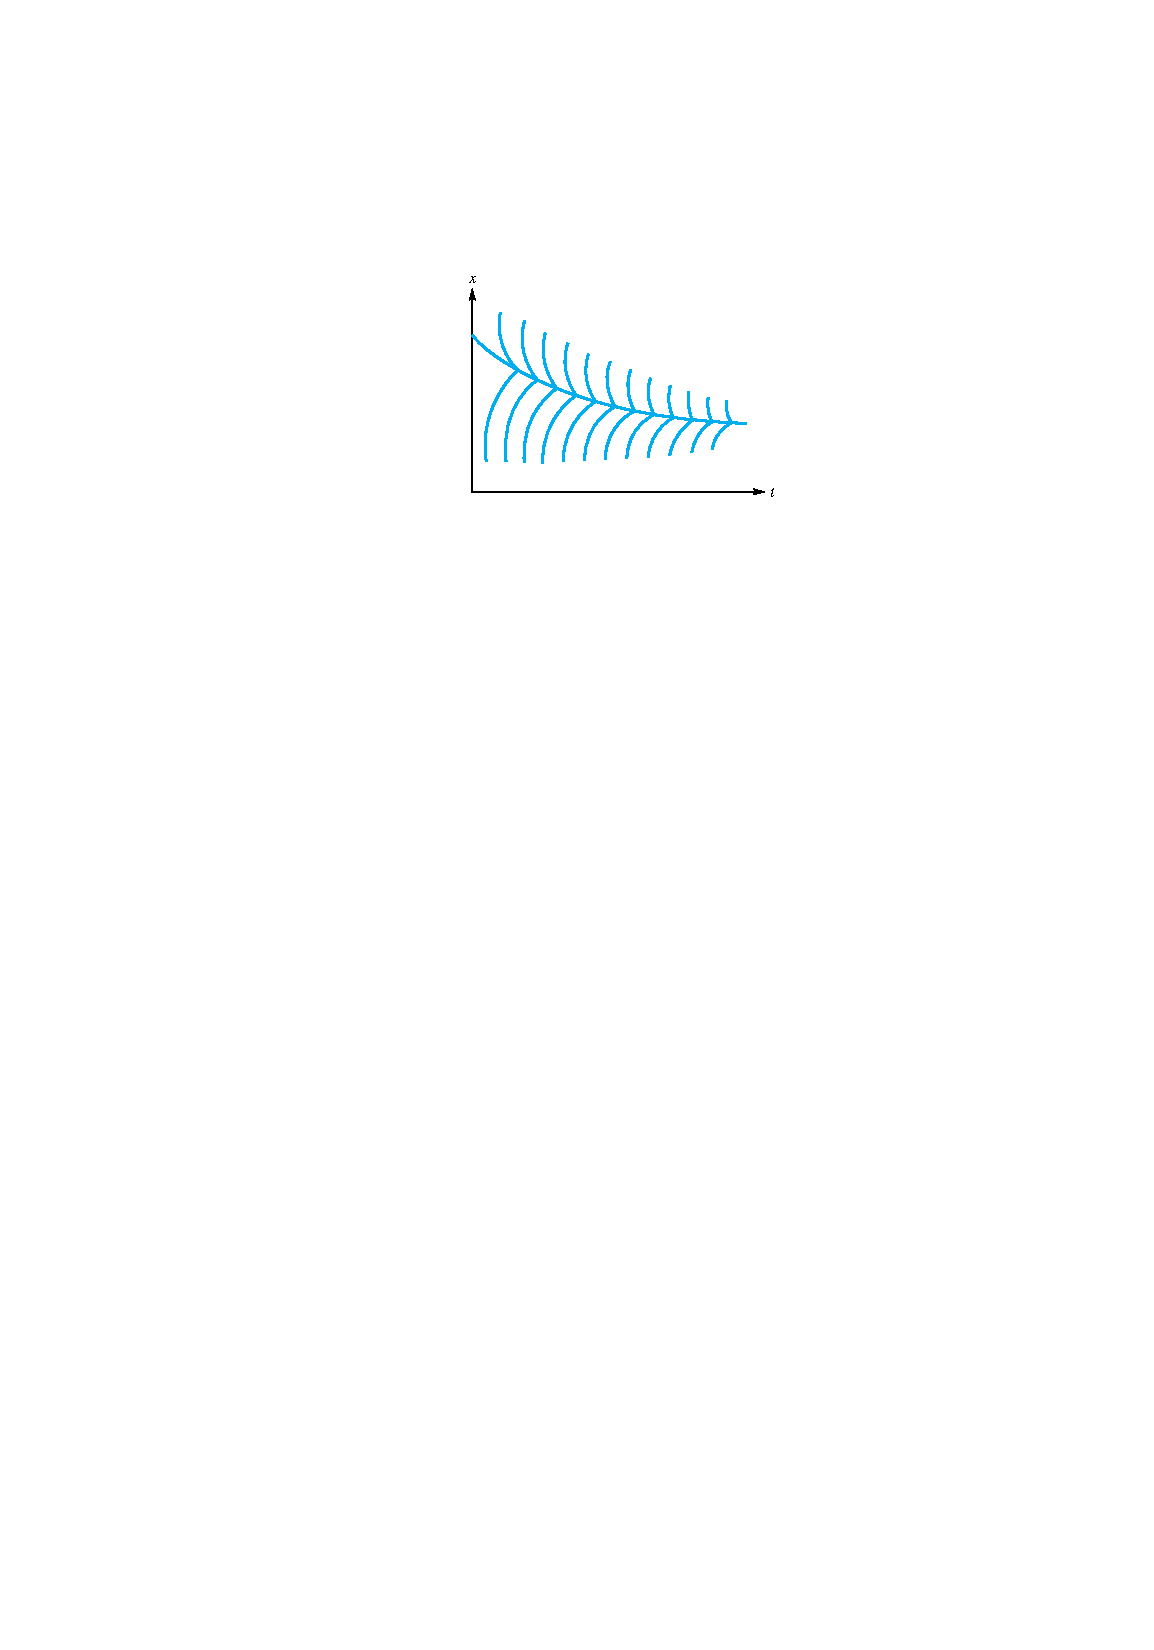
\includegraphics[width=0.8\textwidth]{Lec13_Fig6.pdf}}

 A typical stiff ODE with a slowly
        varying solution surrounded by other solutions with rapidly decaying transients.

\end{frame}

\begin{frame}{Numerical Integration of Stiff ODEs}
    \begin{itemize}
    \item Numerical integration of stiff equations requires special care.
    \item The step size $h$
    needed for stability is determined by the largest eigenvalue $\lambda_{\max}$, even if the terms
    $\exp(-\lambda_{\max}t)$ in the solution decay very rapidly and become insignificant as we move away from $t=0$.
    \end{itemize}
\end{frame}
\begin{frame}{Example I}
    \begin{itemize}
        \item Consider a second order ODE, with initial conditions $x(0)=1$ and $x^{\prime}(0)=0$,
         \[
        x^{\prime \prime}+1001 x^{\prime}+1000 x=0,
        \]
        which can be converted to a system of first-order ODEs
        \[
        \left\{\begin{array}{l}
            x_1^{\prime}=x_2 \\
            x_2^{\prime}=-1000 x_1-1001 x_2
            \end{array}\right..
            \]
            
\item The $\boldsymbol{\Lambda}$ matrix is
\[  
\boldsymbol{\Lambda}=\left[\begin{array}{cc}
0 & -1 \\
1000 & 1001
\end{array}\right]
\]
with eigenvalues $\lambda_1=1$ and $\lambda_2=1000$.
\end{itemize}
\end{frame}
\begin{frame}{Example I (cont.)}
    \begin{itemize}
        \item The solution is
        \[
        \mathbf{x}(t)=C_1 \mathbf{v}_1 \exp(-t)+C_2 \mathbf{v}_2 \exp(-1000 t),
        \]
        where  and $\mathbf{v}_1=[1,-1]^T$ and $\mathbf{v}_2=[1, -1000]^T$.
        \item The solution has two components, one decays rapidly and the other decays slowly.
        \item The problem is stiff.
        \item For Euler's method, the stability condition is $h<2/\lambda_{\max}=2/1000=0.002$.
        \item The Runge-Kutta method would have approximately the same limitation on the step
        size.
    \end{itemize}

\end{frame}
\begin{frame}{Example II}
    \begin{itemize}
        \item Consider a system of ODEs
        $$
\begin{cases}x^{\prime}=-20 x-19 y & x(0)=2 \\ y^{\prime}=-19 x-20 y & y(0)=0\end{cases}
$$
\item The solution
$$
\begin{aligned}
& x(t)=e^{-39 t}+e^{-t} \\
& y(t)=e^{-39 t}-e^{-t}
\end{aligned}
$$
\item The component $\exp(-39t)$ quickly becomes negligible as $t$ increases, starting at 0. 
\item The solution is then approximately given by $x(t)= -y(t)= \exp(-t)$.
\item This function is smooth and decreasing toward 0. A Large step size seems possible.
    \end{itemize}
\end{frame}

\begin{frame}{Example II (cont.)}
    \begin{itemize}
        \item However, using Euler's method, we have
        $$
\begin{array}{ll}
x_{n+1}=x_n+h\left(-20 x_n-19 y_n\right) & x_0=2 \\
y_{n+1}=y_n+h\left(-19 x_n-20 y_n\right) & y_0=0
\end{array}
$$
\item The difference equations can be solved explicitly
\[
\begin{array}{l}
x_{n+1}=\left(1-20 h\right) x_n-19 h y_n \\
y_{n+1}=-19 h x_n+\left(1-20 h\right) y_n
\end{array}
\]
\item For the equations to converge, it is necessary that $h< 2/39 \approx 0.05$.
\item For $x'=-x$, the solution is $x(t)=\exp(-t)$, which is stable for even $h=2$.
    \end{itemize}

\end{frame}
\begin{frame}{Example II (cont.)}
    \begin{itemize}
        \item Let's consider the implicit Euler method instead,
        \item The difference equations are
        $$
\begin{aligned}
& x_{n+1}=x_n+h\left(-20 x_{n+1}-19 y_{n+1}\right) \\
& y_{n+1}=y_n+h\left(-19 x_{n+1}-20 y_{n+1}\right)
\end{aligned},
$$
or in the vector form $\mathbf{X}_{n+1}=\mathbf{X}_n+\mathbf{A} \mathbf{X}_{n+1}$.

\item The solution is
\[
\mathbf{X}_{n+1}=\left(\mathbf{I}-\mathbf{A}\right)^{-1} \mathbf{X}_n.
\]

   
    \end{itemize}
\end{frame}

\begin{frame}{Example II (cont.)}
    
   
\begin{itemize}
     \item The matrix $\mathbf{A}$ is given by
        \[  
        \mathbf{A}=\left[\begin{array}{cc}
        -20h & -19h \\
        -19h & -20h
        \end{array}\right],
        \]
        and $\mathbf{X}_{n}=\left(\mathbf{I}-\mathbf{A}\right)^{-n} \mathbf{X}_0$.
         
        
        \item For $\mathbf{X}_n$ to converge to 0 for any given $\mathbf{X}_0$, it is necessary that the norms of all the eignvalues of $\left(\mathbf{I}-\mathbf{A}\right)$ 
        should be greater than 1. 

    \end{itemize}
\end{frame}
\end{document}


